\documentclass[11pt]{article}

\usepackage[margin=1in]{geometry}
\usepackage{amsmath, amssymb}
\usepackage{graphicx}
\usepackage{booktabs}
\usepackage{caption}
\usepackage{hyperref}
\usepackage{float}
\usepackage{xcolor}

\graphicspath{{figs/}}
\emergencystretch=3em

\newcommand{\todo}[1]{\textcolor{red}{\textbf{[TO WRITE: #1]}}}

\title{MGT 595: Quantitative Investing \\ Problem Set 2}
\author{Group: Ashley Wen, Emily Wu, Grace Gu}
\date{\today}

\begin{document}
\maketitle

\begin{center}
\begin{tabular}{ll}
Ashley Wen & NetID: xw564 \\
Emily Wu   & NetID: esw63 \\
Grace Gu   & NetID: xg325 \\
\end{tabular}
\end{center}

\vspace{1em}

% =====================================================================
\section{Question 1: Mean--Variance Portfolios --- 10 Industries}
% =====================================================================

\paragraph{Data and conventions.} The data are monthly value-weighted returns
on ten U.S.\ industry portfolios from July 1926 to June 2026, giving
$T = 1200$ observations on $N = 10$ industries, with no missing values. All
figures are in percent per month unless stated otherwise: a mean of $1.0584$
means $1.0584\%$ per month. The risk-free rate is the sample mean of the
monthly risk-free column, $r_f = 0.2701\%$ per month. Short sales are
unrestricted, so writing $\mu$ for the vector of sample means, $\Sigma$ for
the sample covariance matrix and $\mathbf{1}$ for a vector of ones,
\begin{equation}
w_{\text{MVP}} = \frac{\Sigma^{-1}\mathbf{1}}{\mathbf{1}'\Sigma^{-1}\mathbf{1}},
\qquad
w_{\text{TAN}} = \frac{\Sigma^{-1}(\mu - r_f\mathbf{1})}
                       {\mathbf{1}'\Sigma^{-1}(\mu - r_f\mathbf{1})},
\label{eq:weights}
\end{equation}
with $\mu_p = w'\mu$, $\sigma_p = \sqrt{w'\Sigma w}$ and
$S_p = (\mu_p - r_f)/\sigma_p$.

\subsection{Question 1(a): MVP, Tangency Portfolio and the Efficient Frontier}

\begin{table}[H]
\centering
\caption{Industry sample moments and the resulting portfolio weights from
equation~\eqref{eq:weights}. Weights sum to one in each column. The last three
rows report the mean, standard deviation and Sharpe ratio of each portfolio.}
\begin{tabular}{lrrrr}
\toprule
 & \multicolumn{2}{c}{Monthly (\%)} & \multicolumn{2}{c}{Weight} \\
\cmidrule(lr){2-3}\cmidrule(lr){4-5}
Industry & Mean & Std.\ Dev. & MVP & Tangency \\
\midrule
NoDur & 0.9402 & 4.5595 & 0.7188 & 0.6645 \\
Durbl & 1.1822 & 8.2136 & $-0.0142$ & 0.1340 \\
Manuf & 1.0385 & 6.2008 & $-0.1905$ & $-0.2242$ \\
Enrgy & 1.0292 & 6.4095 & 0.1527 & 0.2808 \\
HiTec & 1.1699 & 7.1424 & $-0.0621$ & 0.1865 \\
Telcm & 0.8124 & 4.6606 & 0.4889 & 0.1525 \\
Shops & 1.0342 & 5.7802 & $-0.0137$ & 0.0725 \\
Hlth & 1.0680 & 5.5005 & 0.1174 & 0.3530 \\
Utils & 0.8874 & 5.4351 & 0.1293 & 0.0721 \\
Other & 0.9237 & 6.3555 & $-0.3267$ & $-0.6916$ \\
\midrule
\textit{Portfolio mean} (\%/mo) &  &  & 0.8672 & 1.0584 \\
\textit{Portfolio std.\ dev.} (\%/mo) &  &  & 3.8346 & 4.4063 \\
\textit{Sharpe ratio} (monthly) &  &  & 0.1557 & 0.1789 \\
\bottomrule
\end{tabular}
\label{tab:q1a}
\end{table}

\begin{figure}[H]
\centering
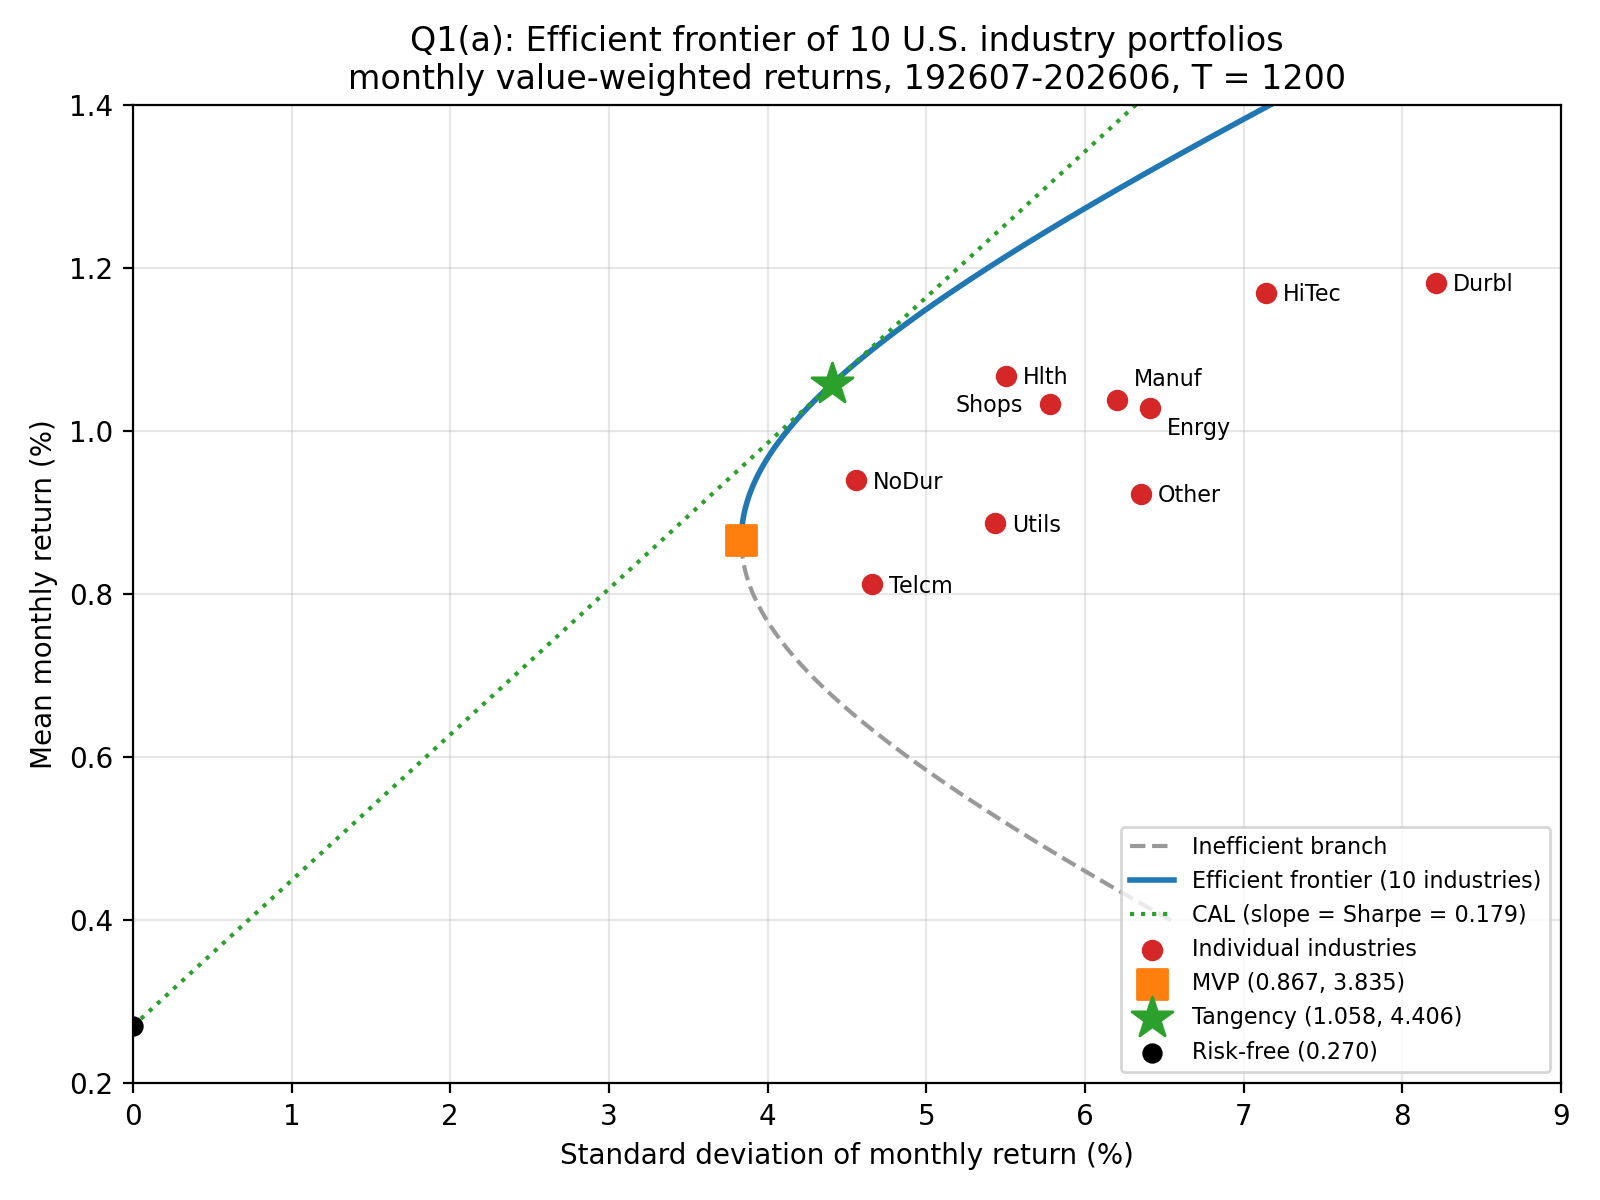
\includegraphics[width=0.72\textwidth]{q1a_frontier.png}
\caption{Efficient frontier of the ten industries in mean--standard deviation
space. Red dots are the individual industries, the orange square is the
minimum variance portfolio, the green star is the tangency portfolio, and the
dotted line is the capital allocation line from the risk-free rate. The dashed
grey curve is the inefficient lower branch.}
\label{fig:q1a}
\end{figure}


\paragraph{Discussion of the weights.}
\begin{itemize}
\setlength{\itemsep}{6pt}\setlength{\parskip}{0pt}

\item \textbf{NoDur is the largest long position in both portfolios}, 0.72 in
the MVP and 0.66 in the tangency portfolio. It has the lowest standard
deviation of the ten industries, 4.56\% per month, and the lowest residual
volatility once the other nine are controlled for. It earns that weight by
hedging the movements the industries share.

\item \textbf{The two portfolios diverge on Telcm}, which the MVP holds at
0.49 and the tangency portfolio at only 0.15. Telcm has the second-lowest
standard deviation but the lowest mean return in the sample, 9.75\% per year.
Minimizing variance alone makes it valuable; once expected return enters, its
low volatility no longer pays for the weakest risk premium of the ten.

\item \textbf{The tangency portfolio is the more aggressive of the two},
despite being long in 8 of 10 industries against 5 for the MVP. Its gross
leverage is 2.83 against 2.21 and its cross-sectional weight dispersion 0.359
against 0.309. The difference is where the extremity sits: the MVP
concentrates on the long side and spreads small shorts across five industries,
three of them negligible, while the tangency portfolio funds eight longs out
of a single short of $-0.69$ in Other, the lowest-Sharpe industry. The extra
leverage is what it costs to bet on mean differences that are small next to an
average pairwise correlation of 0.696.

\end{itemize}

\paragraph{Shape of the frontier.} Minimizing $w'\Sigma w$ subject to
$w'\mu = m$ and $w'\mathbf{1} = 1$ gives first-order conditions that are
linear in $w$, so the optimal weights are an affine function of the target
mean,
\begin{equation}
w(m) = \frac{c - bm}{d}\,\Sigma^{-1}\mathbf{1}
     + \frac{am - b}{d}\,\Sigma^{-1}\mu ,
\end{equation}
with $a = \mathbf{1}'\Sigma^{-1}\mathbf{1}$, $b = \mathbf{1}'\Sigma^{-1}\mu$,
$c = \mu'\Sigma^{-1}\mu$ and $d = ac - b^2$. Substituting back into the
objective gives
\begin{equation}
\sigma^2(m) = \frac{a m^2 - 2bm + c}{d},
\label{eq:frontier}
\end{equation}
a quadratic in $m$, and therefore a parabola in mean--variance space and a
hyperbola in the mean--standard deviation space of Figure~\ref{fig:q1a}. Here
$a = 0.0680$ and $d = 0.000528$, both positive, so the parabola opens toward
higher risk. Three things follow.

\begin{itemize}
\setlength{\itemsep}{6pt}\setlength{\parskip}{0pt}

\item \textbf{The curvature is diversification.} If the industries were
perfectly correlated, combining them would reduce no risk and the attainable
set would be a straight line. Correlations below one bend it leftward, and how
far it bends measures how much diversification is available. Here the average
pairwise correlation is 0.696, so the bend is modest: the MVP standard
deviation of 3.83 is only 15.9\% below NoDur's 4.56, whereas part (c) shows it
would fall to 1.82 if the industries were uncorrelated.

\item \textbf{The vertex is the MVP.} Minimizing the quadratic gives
$m = b/a = 0.8672$ and $\sigma^2 = 1/a = 14.70$, matching the minimum variance
portfolio in Table~\ref{tab:q1a} exactly.

\item \textbf{Dominance makes only the upper branch efficient.} Because
$\sigma^2(m)$ is quadratic, every variance above $1/a$ is attained by two
portfolios, one on each side of the vertex. They carry identical risk but the
lower one returns less, so it is dominated. Since investors prefer a higher
expected return at the same risk, no one would ever hold it: the lower branch
is feasible but never optimal, which is why it is dashed in
Figure~\ref{fig:q1a}.

\end{itemize}

\subsection{Question 1(b): Reliability of the Mean Return Estimates}

The standard error of each sample mean is $\hat\sigma_i/\sqrt{T}$ with
$T = 1200$.

\begin{table}[H]
\centering
\caption{Reliability of the estimated mean returns, annualized. The
$t$-statistic tests the null that the true mean return is zero.}
\begin{tabular}{lrrr}
\toprule
Industry & Mean (\%/yr) & Std.\ Error (\%/yr) & $t$-statistic \\
\midrule
NoDur & 11.28 & 1.58 & 7.14 \\
Durbl & 14.19 & 2.85 & 4.99 \\
Manuf & 12.46 & 2.15 & 5.80 \\
Enrgy & 12.35 & 2.22 & 5.56 \\
HiTec & 14.04 & 2.47 & 5.67 \\
Telcm & 9.75 & 1.61 & 6.04 \\
Shops & 12.41 & 2.00 & 6.20 \\
Hlth & 12.82 & 1.91 & 6.73 \\
Utils & 10.65 & 1.88 & 5.66 \\
Other & 11.08 & 2.20 & 5.03 \\
\bottomrule
\end{tabular}
\label{tab:q1b_rel}
\end{table}

We then raise every estimated mean by one of its own standard errors,
$\tilde\mu_i = \hat\mu_i + \hat\sigma_i/\sqrt{T}$, and recompute the tangency
portfolio. The MVP is unchanged by construction because it does not use $\mu$.

\begin{table}[H]
\centering
\caption{Tangency portfolio weights and statistics before and after raising
every estimated mean by one standard error.}
\begin{tabular}{lrrr}
\toprule
Industry & Baseline & Means $+1$ SE & Change \\
\midrule
NoDur & 0.6645 & 0.5686 & $-0.0960$ \\
Durbl & 0.1340 & 0.1526 & 0.0187 \\
Manuf & $-0.2242$ & $-0.2611$ & $-0.0370$ \\
Enrgy & 0.2808 & 0.2864 & 0.0056 \\
HiTec & 0.1865 & 0.1781 & $-0.0084$ \\
Telcm & 0.1525 & 0.1709 & 0.0184 \\
Shops & 0.0725 & 0.0671 & $-0.0054$ \\
Hlth & 0.3530 & 0.3400 & $-0.0129$ \\
Utils & 0.0721 & 0.0965 & 0.0244 \\
Other & $-0.6916$ & $-0.5991$ & 0.0926 \\
\midrule
\textit{Portfolio mean} (\%/mo) & 1.0584 & 1.1980 & 0.1395 \\
\textit{Portfolio std.\ dev.} (\%/mo) & 4.4063 & 4.3771 & $-0.0292$ \\
\textit{Sharpe ratio} (monthly) & 0.1789 & 0.2120 & 0.0331 \\
\bottomrule
\end{tabular}
\label{tab:q1b_shift}
\end{table}

\begin{figure}[H]
\centering
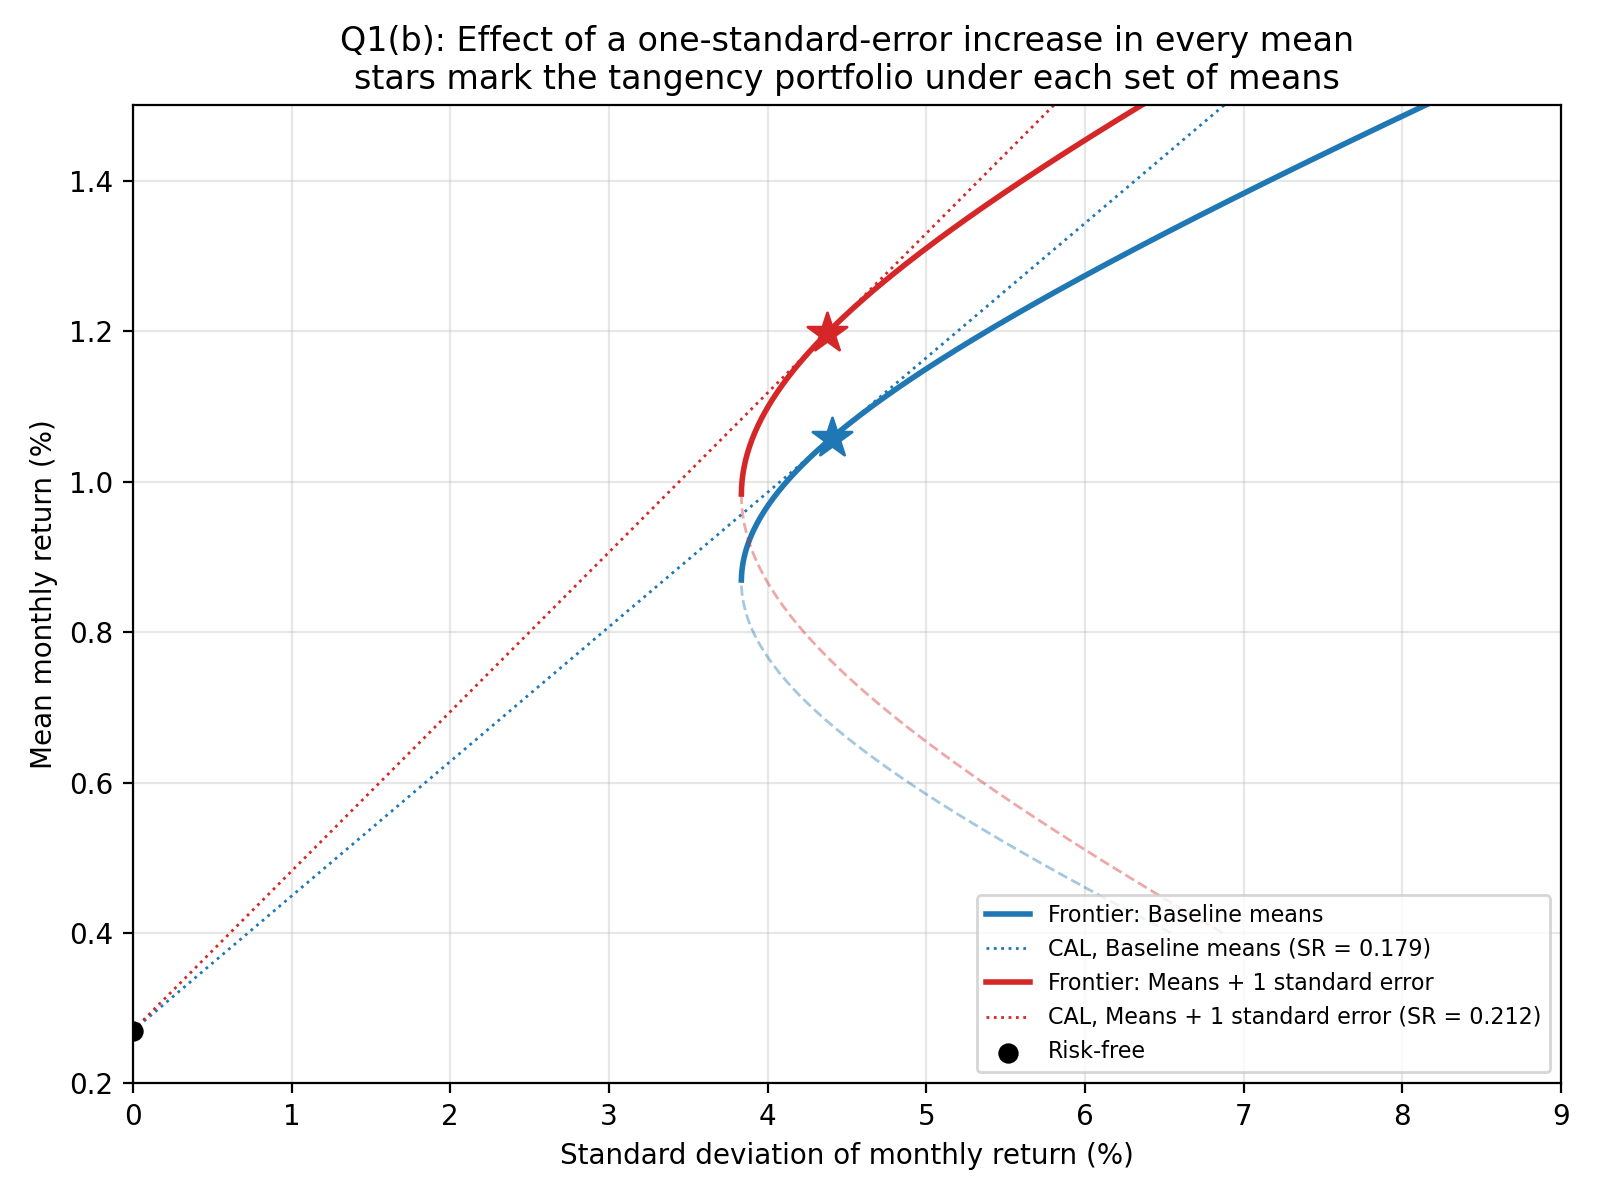
\includegraphics[width=0.72\textwidth]{q1b_frontier_shift.png}
\caption{Efficient frontiers and capital allocation lines under the baseline
means (blue) and after a one-standard-error increase in every mean (red).
Stars mark the tangency portfolio in each case.}
\label{fig:q1b}
\end{figure}

% Numbers available for this discussion:
%   RELIABILITY.  t-statistics run 4.99 to 7.14 against zero, but that is not
%   the test mean-variance optimization depends on: what matters is the
%   cross-sectional spread of the means.  The highest and lowest annual means
%   differ by 4.44 pp while the average standard error is 2.09 pp, so the
%   entire cross-section spans only about 2.1 standard errors.  Testing the
%   extremes directly, Durbl (14.19) minus Telcm (9.75) has t = 1.91 and is
%   NOT significant at 5%, even with a century of data.  The ranking of
%   industries by mean is therefore not statistically identified.
%   HOW MUCH THINGS MOVE.  Weights move moderately: sum|dw| = 0.3192,
%   max|dw| = 0.0960 (NoDur), cosine similarity 0.9953.  The frontier moves a
%   lot: tangency Sharpe 0.1789 -> 0.2120, +18.5%, from a perturbation that is
%   by construction statistically undetectable.
%   CAVEAT worth making: because every mean was raised, much of the shift is a
%   level effect on the frontier; the relative reshuffling of weights is the
%   smaller part of the story.
\paragraph{Discussion.}
\begin{itemize}
\setlength{\itemsep}{6pt}\setlength{\parskip}{0pt}

\item \textbf{The means are not estimated reliably enough to rank the
industries.} Every industry mean is significantly different from zero, with
$t$-statistics from 4.99 to 7.14. Mean--variance optimization needs the
ranking of the industries rather than the level, so we test all 45 pairwise
differences instead, using the standard error of each paired difference
series. Only one is significant at the 5\% level (HiTec minus Telcm,
$t = 2.31$), and 45 tests at that level would throw up about two false
positives by chance. The cross-section therefore looks the same as ten
industries with identical means. We then split the century at 1976 and compare
the two halves. The rank correlation is 0.745, so the extremes do hold up,
with Durbl and HiTec leading in both halves and Telcm trailing in both, while
the middle reshuffles: NoDur moves from ninth to fifth and Manuf from fourth
to seventh.

\item \textbf{The tangency weights move only moderately.} Raising every mean
by one standard error shifts the weight vector by 0.32 in total absolute
terms, the largest single change is 0.096 in NoDur, and the cosine similarity
between the two weight vectors is 0.9953. The composition tilts, and the
direction of the tilt stays the same.

\item \textbf{The frontier moves much more than the weights do.} The tangency
Sharpe ratio rises from 0.1789 to 0.2120, an increase of 18.5\%, and the
capital allocation line shifts with it (Figure~\ref{fig:q1b}). So a
perturbation that no test could detect relocates the whole opportunity set. We
raised every mean at once, so a good part of this is the frontier shifting up
as a whole, and only a smaller part comes from industries changing places.
That is still the point: a century of data does not pin down even the level of
the achievable Sharpe ratio.

\end{itemize}

\subsection{Question 1(c): Reliability of the Covariance Matrix}

We recompute the frontier with the covariances set to zero (keeping the
estimated variances on the diagonal) and then with $\Sigma$ replaced by the
identity matrix. Table~\ref{tab:q1c} reports each portfolio twice: once with
risk measured by the covariance matrix used to build it, and once with the
same weights evaluated under the true sample $\Sigma$. The second measurement
is needed because the assumed risk units are not comparable across the three
cases, and under the identity matrix they are arbitrary.

\begin{table}[H]
\centering
\caption{Portfolio statistics under the three covariance assumptions. The mean
vector $\mu$ is the same in every case. ``Assumed'' measures risk with the
matrix used to construct the weights; ``true'' measures the same weights under
the full sample covariance matrix. Means and standard deviations are monthly
percentages.}
\begin{tabular}{lrrrrr}
\toprule
 & & \multicolumn{2}{c}{Assumed $\Sigma$} & \multicolumn{2}{c}{True $\Sigma$} \\
\cmidrule(lr){3-4}\cmidrule(lr){5-6}
Case & Mean & Std.\ Dev. & Sharpe & Std.\ Dev. & Sharpe \\
\midrule
Full sample --- MVP & 0.8672 & 3.8346 & 0.1557 & 3.8346 & 0.1557 \\
Full sample --- Tangency & 1.0584 & 4.4063 & 0.1789 & 4.4063 & 0.1789 \\
Diagonal --- MVP & 0.9794 & 1.8242 & 0.3888 & 4.8467 & 0.1463 \\
Diagonal --- Tangency & 0.9960 & 1.8455 & 0.3933 & 4.9516 & 0.1466 \\
Identity --- MVP & 1.0086 & 0.3162 & 2.3351 & 5.1422 & 0.1436 \\
Identity --- Tangency & 1.0257 & 0.3199 & 2.3621 & 5.2675 & 0.1434 \\
\bottomrule
\end{tabular}
\label{tab:q1c}
\end{table}

\begin{table}[H]
\centering
\caption{Decomposition of portfolio variance into the contribution of the ten
variance terms and the forty-five covariance terms, using the full sample
covariance matrix. Monthly, in squared percent.}
\begin{tabular}{lrrrr}
\toprule
Portfolio & Total variance & From variances & From covariances & Covariance share \\
\midrule
Equal weighted & 26.442 & 3.741 & 22.701 & 85.9\% \\
MVP & 14.704 & 23.725 & $-9.021$ & $-61.3$\% \\
Tangency & 19.415 & 41.264 & $-21.849$ & $-112.5$\% \\
\bottomrule
\end{tabular}
\label{tab:q1c_decomp}
\end{table}

\begin{figure}[H]
\centering
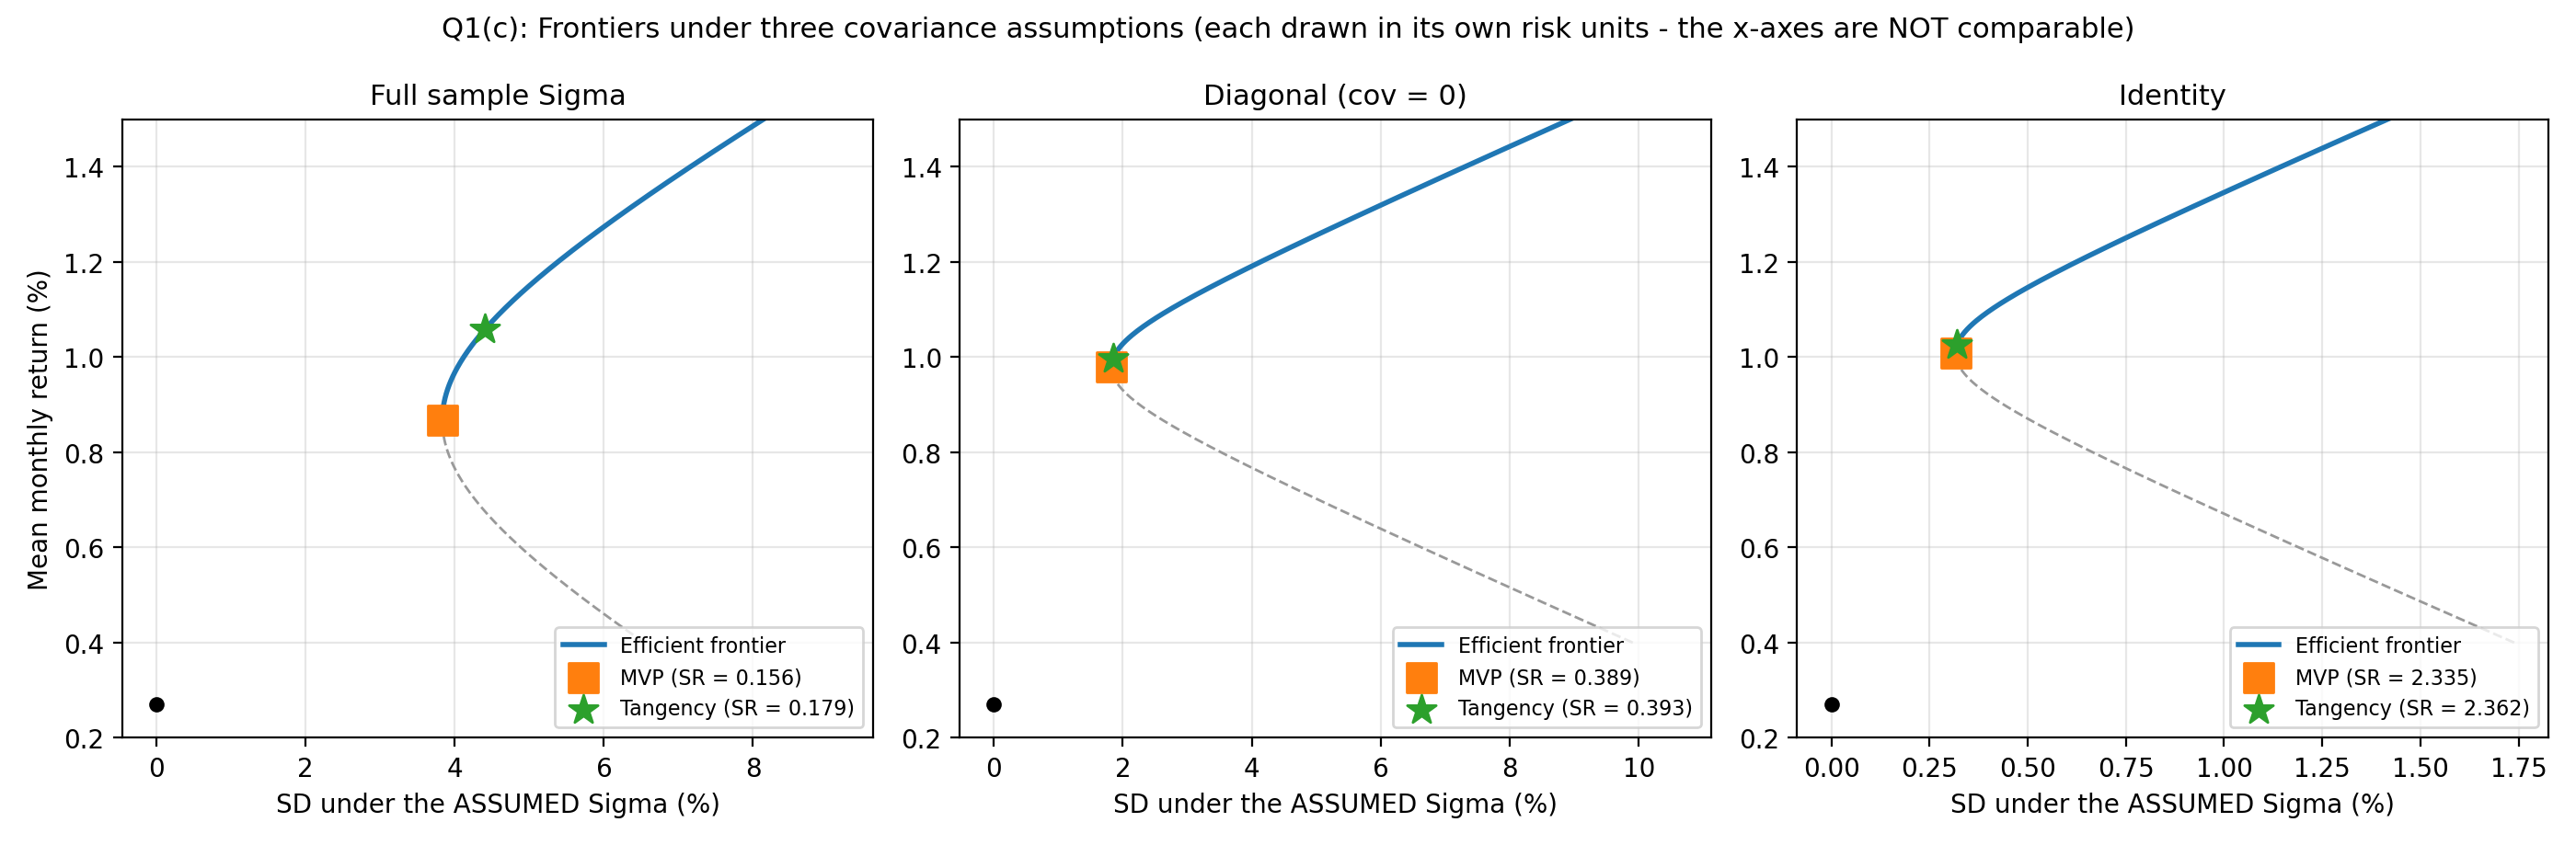
\includegraphics[width=\textwidth]{q1c_frontiers_assumed.png}
\caption{Efficient frontiers under the full sample, diagonal and identity
covariance matrices, each drawn in its own risk units. The horizontal axes are
therefore not comparable across panels.}
\label{fig:q1c}
\end{figure}

% Numbers available for this discussion:
%   RELIABILITY OF SIGMA.  With T = 1200 the covariance matrix is estimated far
%   more precisely than mu (contrast part (b)), but there are 45 covariances to
%   estimate against only 10 variances.
%   SIZE OF THE CHANGE vs part (b).  Under the assumed matrix the frontier
%   moves enormously: tangency Sharpe 0.1789 (full) -> 0.3933 (diagonal) ->
%   2.3621 (identity), far larger than the +18.5% of part (b).  Under the true
%   matrix the ranking reverses: 0.1789 -> 0.1466 -> 0.1434.  So assuming the
%   covariances away makes the portfolio look far better while making it
%   slightly worse.
%   WHY.  Average pairwise correlation is 0.696 (range 0.52-0.90).  Zeroing it
%   fabricates diversification that does not exist, which is why assumed
%   standard deviations collapse from 4.41 to 1.85 to 0.32.
%   COVARIANCES vs VARIANCES.  For the equal-weighted portfolio 85.9% of total
%   variance comes from the covariance terms.  For the MVP and tangency the
%   covariance contribution is negative, because the short positions use the
%   covariances to hedge -- which is exactly why those portfolios cannot be
%   built once covariances are assumed away: the diagonal MVP weights are all
%   positive (0.0493 to 0.1601) and the identity MVP is exactly equal weighted.
\paragraph{Discussion.}
\begin{itemize}
\setlength{\itemsep}{6pt}\setlength{\parskip}{0pt}

\item \textbf{The covariance matrix is estimated precisely, though it is not
stable.} A mean estimate carries 17.2\% relative error on average; a
volatility carries 2.0\%. Monthly returns bounce around five to seven times
more than they drift upward, which makes the mean hard to pin down and leaves
the volatility unaffected. Daily data would sharpen $\Sigma$ further and would
not help $\mu$ at all. Stability is a separate matter: splitting the century
at 1976, average pairwise correlation falls from 0.779 to 0.581, so $\Sigma$
is measured precisely and still moves. The two experiments below set 45
covariances to zero, which is far bigger than any estimation error, so they
test what happens when we assume something wrong rather than when we measure
something badly.

\item \textbf{The frontier changes far more than in part (b).} Measured on its
own assumed risk, the tangency Sharpe ratio goes from 0.1789 to 0.3933 under
the diagonal matrix and to 2.3621 under the identity, against a move of
18.5\% in part (b). We then take the same weights and measure risk with the
real $\Sigma$, which gives 0.1789, 0.1466 and 0.1434. Dropping the covariances
makes the portfolio look much better and leaves it slightly worse.

\item \textbf{The covariance terms matter far more than the variance terms.}
For an equal-weighted portfolio, 85.9\% of total variance comes from the 45
covariance terms rather than the 10 variances. Two results in this section
confirm that.

The first is the shape of the two misspecified frontiers, which look almost
identical to each other. Reaching 0.2 above the MVP costs 2.10 times the MVP's
own risk under the diagonal matrix and 2.04 under the identity, against 1.16
under the real $\Sigma$. Removing the correlations changes everything, and
flattening the variances afterwards changes almost nothing. With real
correlations the ten industries act like 2.26 independent bets, and with
correlations removed they act like 10, which is why the real MVP variance of
14.70 is 4.4 times what it would be with no correlation.

The second is that the damage falls unevenly. Misspecifying $\Sigma$ costs the
MVP 6.0\% and 7.8\% of its true Sharpe ratio, and costs the tangency portfolio
18.1\% and 19.8\%. Under the real $\Sigma$ the tangency portfolio beats the
MVP by 14.9\%, and under the diagonal and identity matrices that edge falls to
0.2\% and $-0.1\%$. Minimizing risk works roughly well with variances alone,
so the MVP survives, while the tangency portfolio's whole edge comes from the
covariances.

\end{itemize}

\subsection{Question 1(d): Jorion Simulation under the Normal Distribution}

Each simulation draws $T = 1200$ monthly return vectors from a multivariate
normal distribution with the historical $\mu$ and $\Sigma$. The MVP and
tangency weights are computed from the \emph{simulated} sample and then
applied to the \emph{actual} industry returns, so the recorded mean and
standard deviation are $w'\mu$ and $\sqrt{w'\Sigma w}$ at the historical
moments. This is the essential feature of the Jorion (1986) design: the
weights carry estimation error but are judged against the true distribution.
The experiment is repeated 1{,}000 times.

\begin{table}[H]
\centering
\caption{Estimation error across 1{,}000 simulations, for both Question 1(d)
and Question 1(e). Portfolio means and standard deviations are evaluated on
the actual industry returns, in percent per month. ``SD of weights'' is the
cross-simulation standard deviation of a portfolio weight, averaged over the
ten industries.}
\begin{tabular}{lrrrrr}
\toprule
 & \multicolumn{2}{c}{Portfolio mean} & \multicolumn{2}{c}{Portfolio std.\ dev.} & \\
\cmidrule(lr){2-3}\cmidrule(lr){4-5}
Experiment & Average & Std.\ dev. & Average & Std.\ dev. & SD of weights \\
\midrule
Normal --- MVP & 0.8671 & 0.0096 & 3.8489 & 0.0066 & 0.0381 \\
Normal --- Tangency & 1.0650 & 0.0793 & 4.9938 & 0.6388 & 0.2716 \\
Bootstrap --- MVP & 0.8693 & 0.0176 & 3.8627 & 0.0142 & 0.0523 \\
Bootstrap --- Tangency & 1.0692 & 0.0802 & 5.0046 & 0.6377 & 0.2703 \\
\bottomrule
\end{tabular}
\label{tab:q1de}
\end{table}

\begin{figure}[H]
\centering
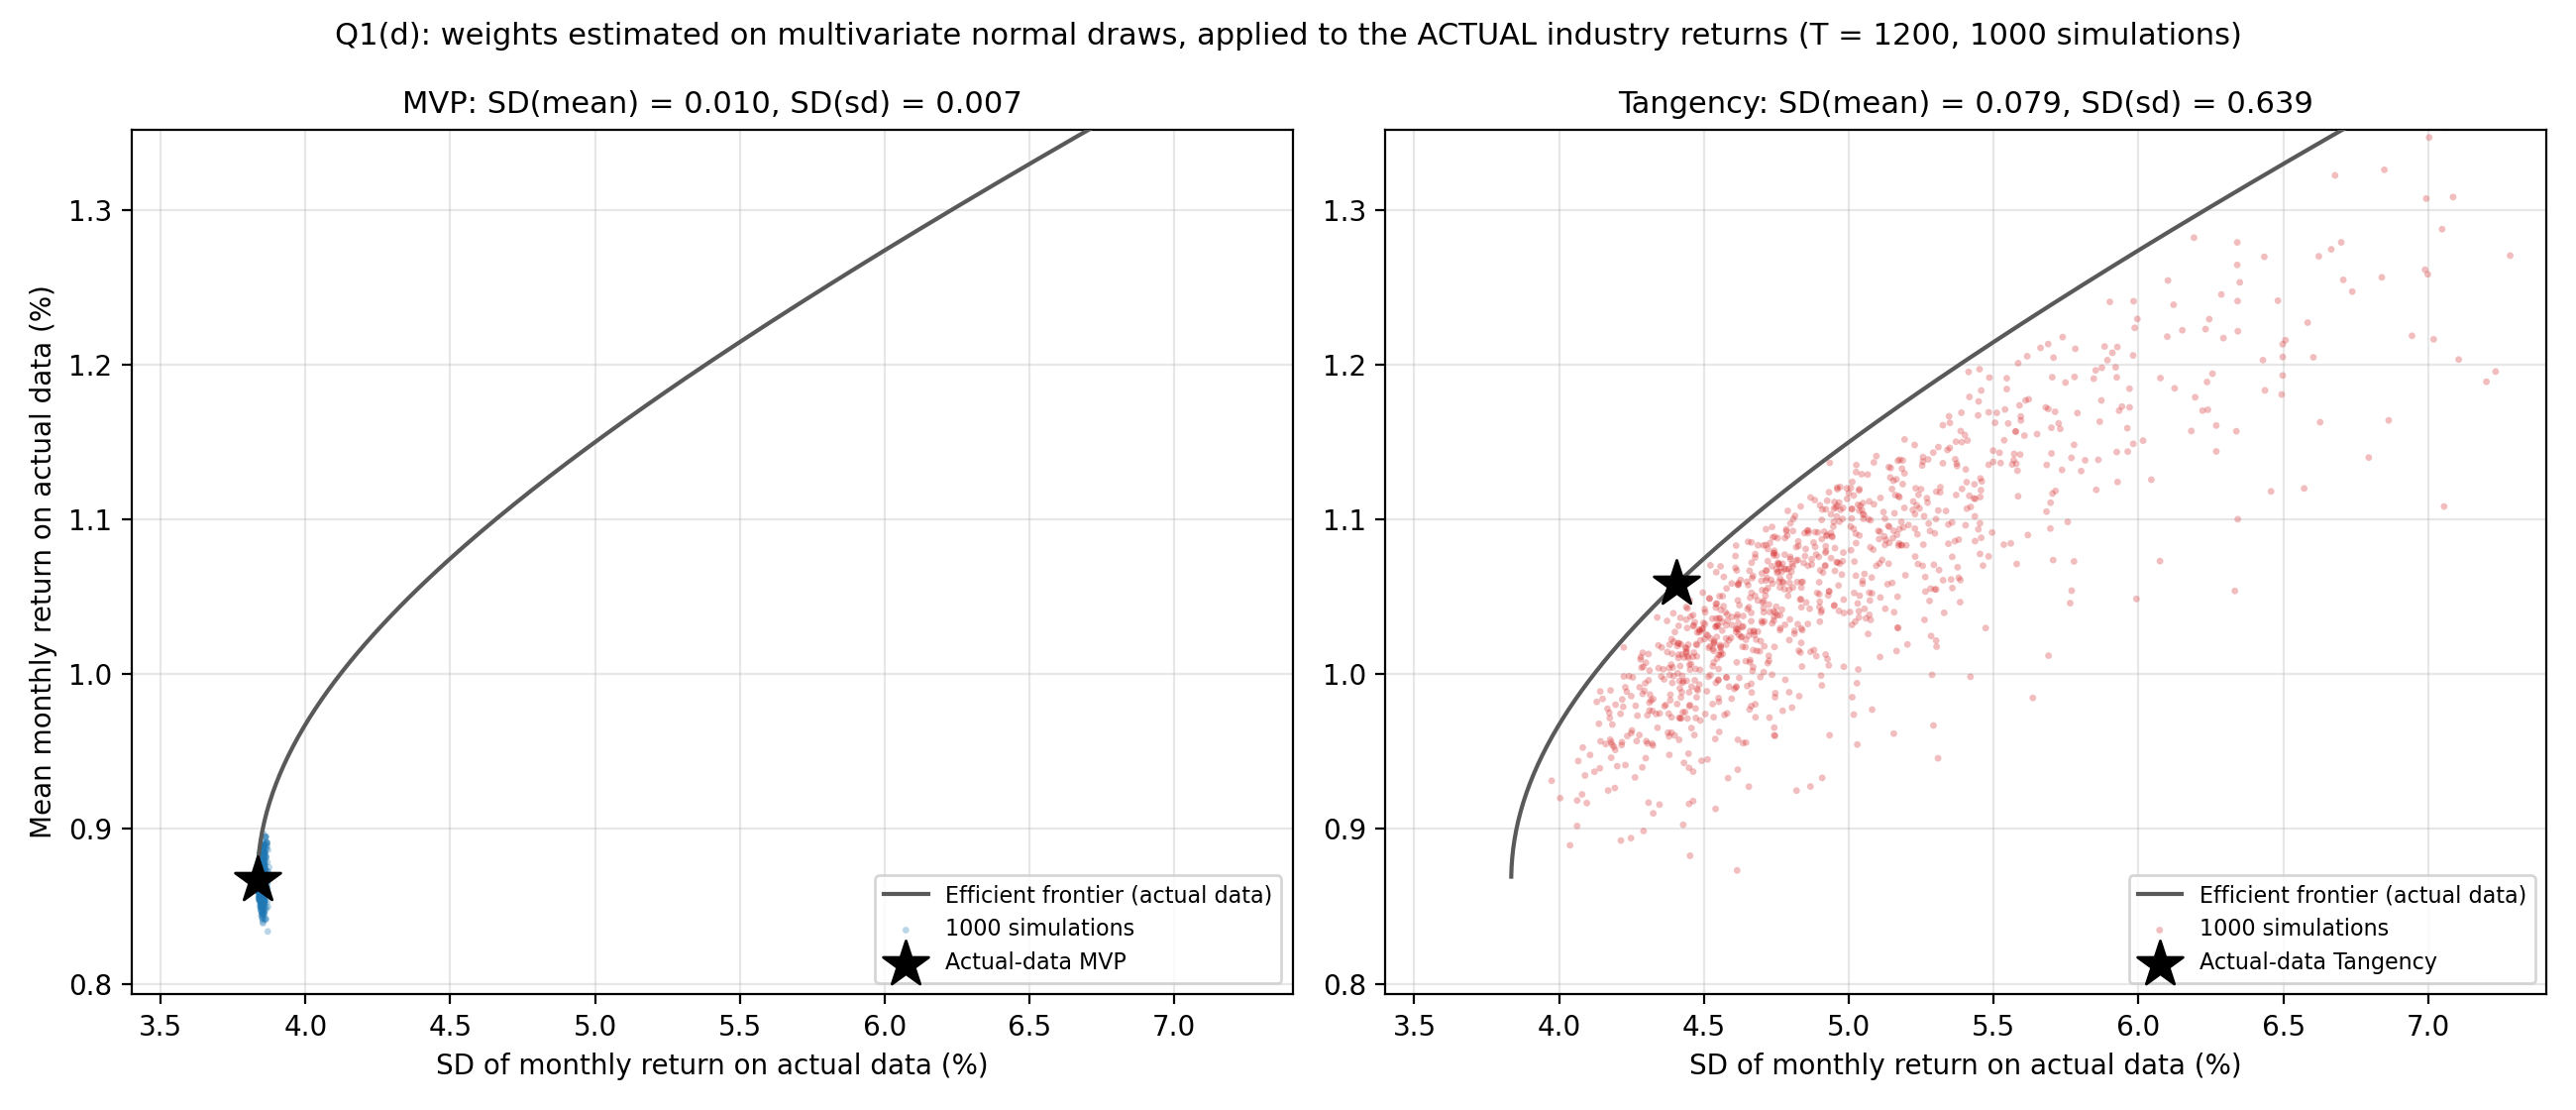
\includegraphics[width=\textwidth]{q1d_normal_clouds.png}
\caption{Question 1(d). Each point is one of 1{,}000 simulations: weights
estimated from a multivariate normal sample of $T = 1200$ months, then applied
to the actual industry returns. The black star is the portfolio built from the
actual data. Both panels share the same axes.}
\label{fig:q1d}
\end{figure}

% Numbers available for this discussion:
%   - Tangency cloud is 8.3x wider than the MVP cloud in realized mean and
%     96.3x wider in realized standard deviation (normal simulation).
%   - Average cross-simulation SD of a weight: 0.0381 (MVP) vs 0.2716
%     (tangency), a factor of about 7.
%   - WHY: w_MVP depends only on Sigma, which is estimated precisely; w_TAN
%     depends on Sigma^{-1}(mu - rf), and mu has very poor signal-to-noise
%     (part (b)).  The near-singular Sigma then amplifies that noise.
%   - The tangency cloud sits to the RIGHT of the frontier: the average
%     simulated tangency portfolio has sd 4.99 against 4.41 for the
%     actual-data tangency portfolio, so estimation error costs real
%     out-of-sample performance.
\paragraph{Discussion.}
\todo{state which portfolio is estimated with less error, and why}

\paragraph{AI Integration --- Simulation code generation.}

\textit{Prompt:}
\todo{paste the exact prompt given to the LLM}

\textit{What we had to fix or adjust:}
\todo{list the corrections}

% This is the graded observation.  If the LLM evaluated the weights on the same
% simulated data used to estimate them, our own runs quantify the error: doing
% so raises the average tangency Sharpe ratio from 0.1599 to 0.1991, an
% overstatement of 24.5%, while the MVP is barely affected (0.1551 vs 0.1561,
% 0.6%).  The in-sample mistake is therefore specifically a tangency problem.
\textit{Did the LLM apply the simulated weights to the actual returns?}
\todo{state explicitly whether the LLM made the in-sample mistake}

\textit{Did the LLM correctly predict which portfolio has smaller estimation
error, and does its economic explanation hold up?}
\todo{evaluate the LLM's prediction and reasoning}

\subsection{Question 1(e): Empirical Row Bootstrap Simulation}

We repeat the experiment under the empirical distribution. Each simulation
draws $T = 1200$ month indices uniformly with replacement from
$\{1, \ldots, T\}$ and takes the corresponding rows of the actual return
matrix, so all ten industry returns for a sampled month stay together.
Sampling whole rows preserves the contemporaneous cross-sectional dependence
and the non-normal shape of the marginal distributions, while destroying
serial dependence such as volatility clustering. As before, weights are
estimated on the bootstrap sample and applied to the actual returns, 1{,}000
times. Results are in Table~\ref{tab:q1de} alongside the normal simulation.

\begin{figure}[H]
\centering
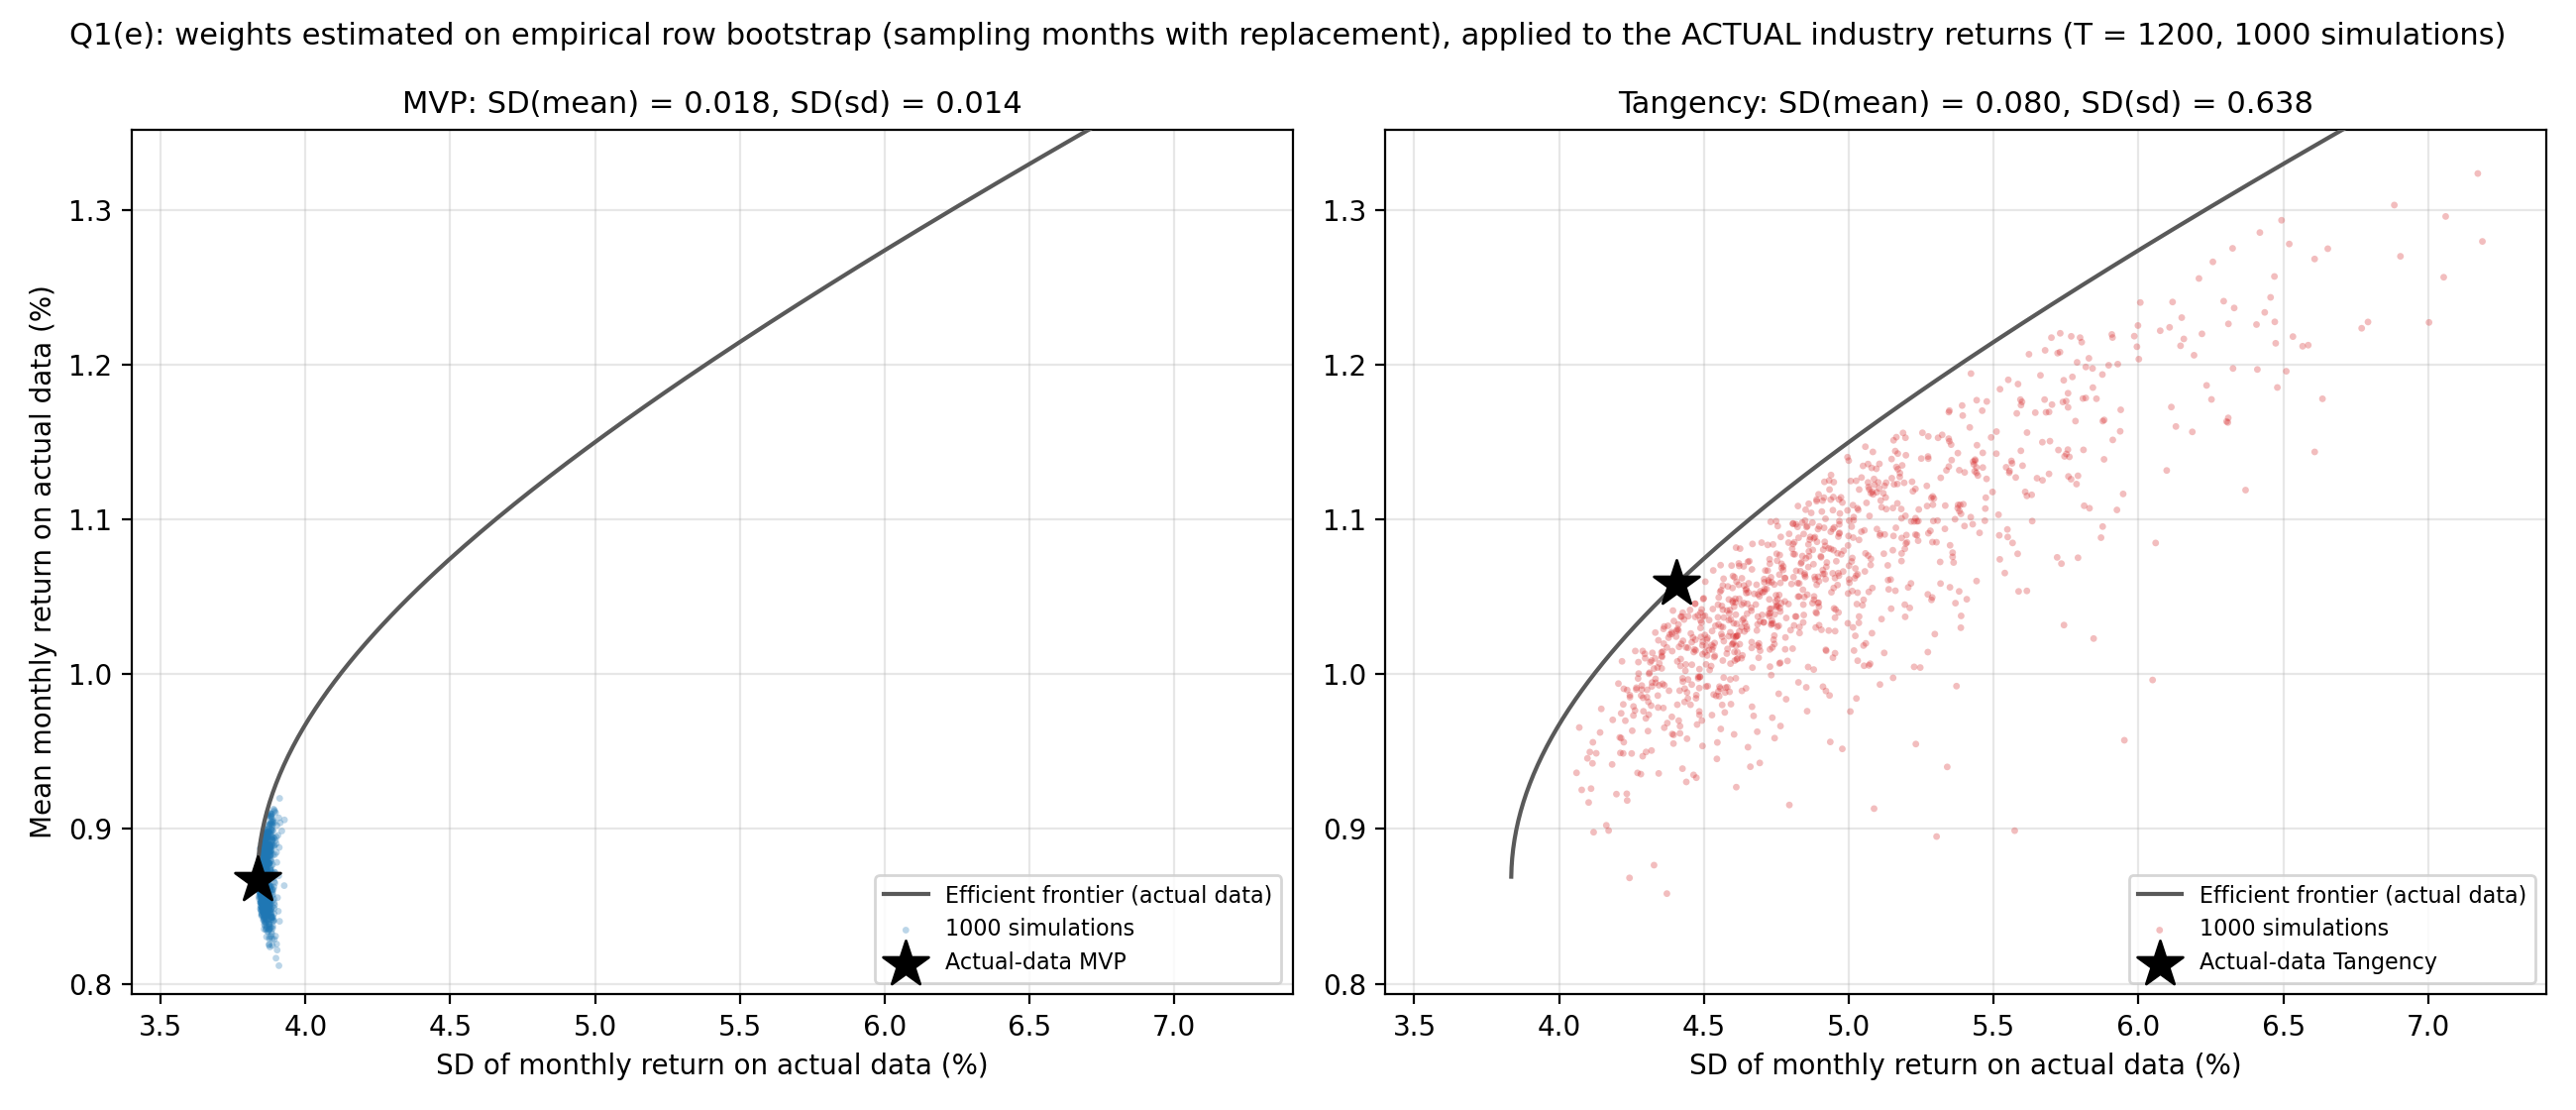
\includegraphics[width=\textwidth]{q1e_bootstrap_clouds.png}
\caption{Question 1(e). Weights estimated on empirical row-bootstrap samples
and applied to the actual industry returns, 1{,}000 simulations. Axes are
identical to Figure~\ref{fig:q1d} so the two experiments can be compared
directly.}
\label{fig:q1e}
\end{figure}

% Numbers available for this discussion:
%   - The answer is asymmetric, which is the interesting part:
%       MVP:      bootstrap dispersion is 1.83x the normal in realized mean
%                 and 2.14x in realized standard deviation.
%       Tangency: 1.01x and 1.00x, essentially unchanged.
%   - Interpretation: fat tails and skewness in actual monthly returns hurt the
%     covariance estimate that drives the MVP, so the MVP cloud widens.
%     Tangency error is already dominated by noise in mu-hat, so switching from
%     the normal to the empirical distribution adds nothing on top.
%   - The ordering is unchanged: the tangency cloud is still far wider than the
%     MVP cloud under the bootstrap (4.6x in mean, 45.0x in standard deviation).
%   - Limitation worth naming: the row bootstrap treats months as i.i.d., so it
%     ignores volatility clustering; a block bootstrap would relax this.
\paragraph{Discussion.}
\todo{compare estimation error under the bootstrap with the normal simulation
of part (d)}

% =====================================================================
% Question 2 (three-asset hand calculation) and Question 3 (robust
% portfolio construction) are written by the other group members.  Paste
% them in below as \section{...} blocks before \end{document}.
% =====================================================================

\end{document}
